\documentclass[11pt]{article}

\usepackage[margin=1in]{geometry}
\usepackage[T1]{fontenc}
\usepackage{lmodern}
\usepackage{amsmath}
\usepackage{booktabs}
\usepackage{graphicx}
\usepackage{enumitem}
\usepackage{xcolor}
\usepackage[hidelinks]{hyperref}

\setlist{itemsep=2pt, topsep=4pt}
\setlength{\emergencystretch}{2em}
\newcommand{\code}[1]{\texttt{#1}}

\title{Compositional Inconsistency as a Verification Signal:\\Pilot Results on MuSiQue}
\author{William Betts\\[2pt]\small Building on the verification-budget framework of Allison Li}
\date{11 November 2026}

\begin{document}
\maketitle

\begin{abstract}
Compositional inconsistency is the case where a model answers a multi-hop question
differently in one step than step by step. It predicts errors on short chains and in
weaker models, but as pre-specified it does not add predictive value beyond confidence and
self-consistency at scale. We sampled both routes on MuSiQue chain questions with three
OpenAI models (gpt-4.1, gpt-4.1-mini, gpt-5.5), labelled every claim against gold answers,
and scored selection strategies under the parent project's fixed verification budget (25\%
of claims checked, swept from 6\% to 63\%). On 100 two-hop questions, composition was the
best non-oracle strategy for all three models, and for gpt-4.1-mini it raised
error-prediction AUROC by $+0.139$ (95\% CI $+0.035$ to $+0.250$). On 300 questions with
2-, 3- and 4-hop chains, the pre-specified score (maximum over chain regions) showed no gain
for either gpt-4.1-mini ($+0.001$) or gpt-5.5 ($-0.007$). An exploratory diagnosis traces
much of the gpt-4.1-mini null to that aggregator: the full-chain score recovers a $+0.053$
gain on 3--4 hop chains (CI $+0.006$ to $+0.102$). Stated confidence was near chance in
every open-book run (AUROC 0.48--0.60). These are pilot results on MuSiQue train; the
full-chain hypothesis needs pre-registration and a held-out test.
\end{abstract}

\section{Introduction}

The question is whether a structural signal the model cannot misreport can tell a verifier
where to spend a limited checking budget better than the model's own confidence. This
extends the parent project by Allison Li
(\href{https://github.com/allison324/think-before-you-trust}{think-before-you-trust}), which
models reasoning as a claim DAG. A check reveals one claim's truth, a caught false claim
quarantines everything downstream, and strategies compete under a fixed number of checks.
Her simulations use synthetic DAGs with error and propagation rates fitted to PARC (base
error 0.176, propagation 0.750). Two of her research questions frame this work:
\begin{enumerate}
  \item Does self-reported confidence help pick which claims to verify under a limited budget?
  \item When confidence is unreliable, is there a structural signal that performs comparably?
\end{enumerate}

The signal tested here comes from category theory. For a chain
$x \xrightarrow{f} y \xrightarrow{g} z$, a structure-preserving system satisfies
\begin{equation}
  F(g \circ f)(x) = F(g)\bigl(F(f)(x)\bigr).
\end{equation}
Answering the composite question directly should therefore agree with answering $f$,
feeding the model's own answer into $g$, and answering $g$. The composition score is the
total variation distance between the two routes' answer distributions,
\begin{equation}
  \delta_{\text{comp}} = d_{\mathrm{TV}}\bigl(P_{\text{direct}}(a \mid x),\, P_{\text{stepwise}}(a \mid x)\bigr),
\end{equation}
and needs no gold answers. The experiment replaces her synthetic DAGs with real MuSiQue
chains and real model outputs. It keeps her budget, quarantine rule and reliability metric
unchanged, so results are directly comparable to her strategy tables.

\section{Methodology}

Each question runs through six stages. Only the labelling stage reads gold answers, so every
detector signal is gold-free.

\subsection{Data}
\begin{itemize}
  \item \textbf{Source:} MuSiQue-Ans v1.0 \emph{train}, linear chains only (step $k$ refers
        to exactly step $k-1$). Dev and test stay untouched for a later held-out study.
  \item \textbf{pilot100:} 100 two-hop chains (seed 0), the same questions as the ongoing
        Groq gpt-oss-120b pilot.
  \item \textbf{scale300:} 100 each of 2-, 3- and 4-hop chains. The same seed makes its
        two-hop third identical to pilot100.
  \item \textbf{Condition:} open book by default, so every call sees the same 20 MuSiQue
        paragraphs (evidence plus distractors). Closed book drops them.
  \item \textbf{Audit:} all questions kept, matching the pilot audit. Pre-registered flags
        (awkwardly rendered hops, time-sensitive wording) are recorded but not yet reviewed
        by hand.
\end{itemize}

\subsection{Per-question probes}
\begin{enumerate}
  \item \textbf{Original output (1 call):} final answer, an answer per step, and a stated
        confidence (0--100).
  \item \textbf{Direct route:} $N$ samples of the composite question.
  \item \textbf{Stepwise route:} $N$ chains that ask step 1, substitute the model's own
        answer into step 2, and so on.
  \item \textbf{Same-route control:} a second independent batch of both routes, so ordinary
        sampling noise is measured.
  \item \textbf{Self-consistency:} $3N$ samples of the original question, matched to the
        probe's call count.
\end{enumerate}
$N = 3$ unless stated, and the temperature is 0.7 for every model. Longer chains get one
region per adjacent pair of steps plus the full chain. Sub-regions use a composite built by
nesting the step questions, since MuSiQue only writes the full composite.

\subsection{Signals}
\begin{center}
\small
\begin{tabular}{lll}
\toprule
Signal & Definition & Source \\
\midrule
Confidence & stated confidence, reversed & self-report \\
Self-consistency & $1 -$ modal share over $3N$ samples & sampling \\
Same-route noise & mean $d_{\mathrm{TV}}$ between the two batches of each route & sampling \\
Composition (\code{delta\_comp\_max}) & max over regions of $d_{\mathrm{TV}}$(direct, stepwise) & structure \\
\bottomrule
\end{tabular}
\end{center}
Answers are compared after SQuAD-style normalisation (exact match). Abstentions and
unparseable replies are kept as explicit outcomes.

\subsection{Labels}
Every step answer and the final answer are labelled against MuSiQue references. An answer is
correct at token F1 $\geq 0.8$ (aliases allowed for the final answer) and false otherwise.
Abstentions are reported separately and left out of the primary analysis.

\subsection{Analyses}
\begin{itemize}
  \item \textbf{H1 (prediction):} two logistic regressions with 5-fold out-of-fold
        predictions. The baseline uses confidence, hop count, question length,
        self-consistency and same-route noise; the augmented model adds composition. We
        report the AUROC gain with a 2,000-iteration paired bootstrap 95\% CI.
  \item \textbf{H2 (localisation):} AUROC of composition ranking regions that contain a
        false claim above clean regions.
  \item \textbf{Fixed budget (Stage F):} the parent project's evaluation on real chains.
        Each step is a node, and a strategy checks the top $B$ claims. A caught false claim
        quarantines the later steps of its question, and
        \begin{equation}
          \text{reliability} = 1 - \frac{\text{undetected false claims}}{\text{total claims}}.
        \end{equation}
        The headline $B$ is 25\% of claims (her 20 checks of 80 nodes), swept over her 5 to
        50 of 80. Strategies are Random (floor, 500 draws), her uncertainty-first and
        dependency-aware rules ($p_{\text{false}} \cdot D$, with $D = 1 +$ downstream
        claims), self-consistency${}\cdot D$, composition${}\cdot D$, learned
        baseline${}\cdot D$, learned + composition${}\cdot D$, and Oracle (ceiling).
        Differences carry a 1,000-iteration paired bootstrap over questions.
\end{itemize}

\subsection{Run grid}
\begin{center}
\small
\begin{tabular}{lllll}
\toprule
Task set & Model & Condition & $N$ & Questions \\
\midrule
pilot100 & gpt-4.1 & open & 3 & 100 \\
pilot100 & gpt-4.1-mini & open & 3, 5, 10 & 100 \\
pilot100 & gpt-4.1-mini & closed & 3 & 100 \\
pilot100 & gpt-5.5 & open & 3, 5 & 100 \\
pilot100 & gpt-5.5 & closed & 3 & 100 \\
scale300 & gpt-4.1-mini & open & 3 & 300 \\
scale300 & gpt-5.5 & open & 3 & 300 \\
\bottomrule
\end{tabular}
\end{center}
gpt-5.5 runs with \code{reasoning\_effort: none}, the only setting in which it accepts
temperature 0.7.

\section{Results}

Composition wins the fixed-budget comparison on two-hop pilots, but its pre-specified form
adds nothing once 3- and 4-hop chains are included. All numbers come from cached runs
replayed with deterministic scoring.

\subsection{Error prediction (H1)}
Table~\ref{tab:h1} gives each signal's AUROC alone (0.5 is chance) and the AUROC gain from
adding composition to the baseline predictor.

\begin{table}[h]
\centering
\small
\caption{Single-signal AUROC and H1 gain (95\% CI).}
\label{tab:h1}
\begin{tabular}{lrrrrrrl}
\toprule
Run & $n$ & Err. & Conf. & SC & Noise & Comp. & H1 gain \\
\midrule
pilot100 $\cdot$ gpt-4.1-mini & 96 & 34\% & 0.48 & 0.64 & 0.59 & \textbf{0.67} & $\mathbf{+0.139}$ [+0.035, +0.250] \\
pilot100 $\cdot$ gpt-4.1 & 100 & 30\% & 0.53 & 0.63 & 0.66 & 0.57 & $-0.026$ [$-0.064$, +0.009] \\
pilot100 $\cdot$ gpt-5.5 & 100 & 34\% & 0.57 & 0.63 & 0.64 & 0.63 & $+0.001$ [$-0.069$, +0.064] \\
scale300 $\cdot$ gpt-4.1-mini & 292 & 40\% & 0.52 & 0.67 & 0.62 & 0.60 & $+0.001$ [$-0.033$, +0.036] \\
scale300 $\cdot$ gpt-5.5 & 300 & 32\% & 0.60 & 0.63 & 0.64 & 0.58 & $-0.007$ [$-0.022$, +0.008] \\
\bottomrule
\end{tabular}
\end{table}

Stated confidence is close to chance in every open-book run. The one significant H1 gain,
gpt-4.1-mini on two-hop chains, does not survive the move to 300 mixed-length questions.

\subsection{Fixed verification budget}
Table~\ref{tab:budget} gives reliability at a budget of 25\% of claims. On pilot100,
composition beat the parent project's dependency-aware rule by $+0.045$ (gpt-4.1-mini),
$+0.049$ (gpt-4.1, CI $+0.010$ to $+0.090$) and $+0.017$ (gpt-5.5).

\begin{table}[h]
\centering
\small
\caption{Reliability at a 25\% verification budget.}
\label{tab:budget}
\begin{tabular}{lrrrrrrr}
\toprule
Run & Random & Dep.-aware & SC & Comp. & Learned & Learned+C & Oracle \\
\midrule
pilot100 $\cdot$ gpt-4.1-mini & 0.728 & 0.755 & 0.740 & \textbf{0.790} & 0.750 & 0.770 & 0.940 \\
pilot100 $\cdot$ gpt-4.1 & 0.826 & 0.835 & 0.865 & \textbf{0.870} & 0.860 & 0.860 & 1.000 \\
pilot100 $\cdot$ gpt-5.5 & 0.825 & 0.840 & 0.845 & \textbf{0.855} & 0.820 & 0.840 & 1.000 \\
scale300 $\cdot$ gpt-4.1-mini & 0.756 & 0.790 & 0.753 & 0.777 & \textbf{0.796} & 0.792 & 1.000 \\
scale300 $\cdot$ gpt-5.5 & 0.850 & \textbf{0.862} & 0.860 & 0.854 & 0.852 & 0.857 & 1.000 \\
\bottomrule
\end{tabular}
\end{table}

At scale the strategies bunch together: the non-random spread is 0.010 for gpt-5.5 and 0.043
for gpt-4.1-mini, where the learned baseline leads. Composition no longer beats
dependency-aware (gpt-5.5: $-0.015$, CI $-0.032$ to $+0.002$). Across the full sweep (6\% to
63\% of claims) no strategy dominates at scale. The leader changes with budget, and the
non-oracle strategies stay within 0.045 of each other at every point. Oracle sits below 1.0
for gpt-4.1-mini on pilot100 because it has more false claims than checks.

\subsection{Chain length}
Composition carries its signal on two-hop chains and fades with length, while confidence
improves with length for gpt-5.5 (Table~\ref{tab:hops}).

\begin{table}[h]
\centering
\small
\caption{Single-signal AUROC by chain length, scale300.}
\label{tab:hops}
\begin{tabular}{lrrrrr}
\toprule
Model & Hops & Err. & Conf. & SC & Comp. (max) \\
\midrule
gpt-4.1-mini & 2 & 34\% & 0.48 & 0.64 & 0.67 \\
gpt-4.1-mini & 3 & 40\% & 0.52 & 0.69 & 0.55 \\
gpt-4.1-mini & 4 & 47\% & 0.53 & 0.68 & 0.52 \\
gpt-5.5 & 2 & 34\% & 0.57 & 0.63 & 0.63 \\
gpt-5.5 & 3 & 33\% & 0.62 & 0.62 & 0.60 \\
gpt-5.5 & 4 & 28\% & 0.65 & 0.66 & 0.56 \\
\bottomrule
\end{tabular}
\end{table}

\subsection{Localisation (H2)}
Composition ranks regions containing a false claim above clean ones with AUROC 0.64
(gpt-5.5) and 0.59 (gpt-4.1-mini), across 600 regions each. The top 10\% of regions are 58\%
and 73\% erroneous respectively, but they cover only 16\% and 13\% of all erroneous claims.

\subsection{Samples per route}
More samples do not sharpen the signal. For gpt-4.1-mini on pilot100 the H1 gain is $+0.139$
at $N = 3$, $+0.124$ at $N = 5$ and $+0.143$ at $N = 10$, with composition AUROC flat at
0.67--0.68. gpt-5.5 at $N = 5$ stays null ($-0.024$).

\subsection{Closed book}
Without documents, errors rise to 71\% (gpt-4.1-mini) and 68\% (gpt-5.5). Confidence becomes
the best single signal (AUROC 0.73 and 0.65), and composition adds nothing ($-0.013$ and
$-0.007$). The composition signal is about how a model chains evidence it reads, not about
what it knows.

\subsection{Inconsistent but correct}
At scale, 125 (gpt-4.1-mini) and 126 (gpt-5.5) of 300 questions show route disagreement
despite a correct final answer. Only 13 and 20 are wrong with both routes agreeing. Part of
this is exact-match answer identity: ``May 2, 2008'' and ``May 2'' count as different
answers.

\subsection{Cost}
A two-hop question costs about 28 calls and 66k prompt tokens. The 300-question sets average
61 calls per question (45M prompt tokens per model). Every response is cached, so
reanalysis is free.

\section{Exploratory finding: the aggregator hides the signal}

Much of the gpt-4.1-mini null at scale comes from taking the maximum over regions, not from
an absent signal. On 3- and 4-hop chains, sub-regions are asked through synthetic nested
composites (``What is the county of (the answer to \ldots)?''). Those read poorly and come
out inconsistent almost every time. For gpt-4.1-mini the mean sub-region score is 0.74 on
3-hop and 0.91 on 4-hop chains, against 0.57 and 0.69 for the full chain, whose direct
question is MuSiQue's human-written one. The maximum is then close to saturated and carries
little information (AUROC 0.52--0.55 for gpt-4.1-mini on 3--4 hop chains;
Figure~\ref{fig:agg}).

\begin{figure}[h]
\centering
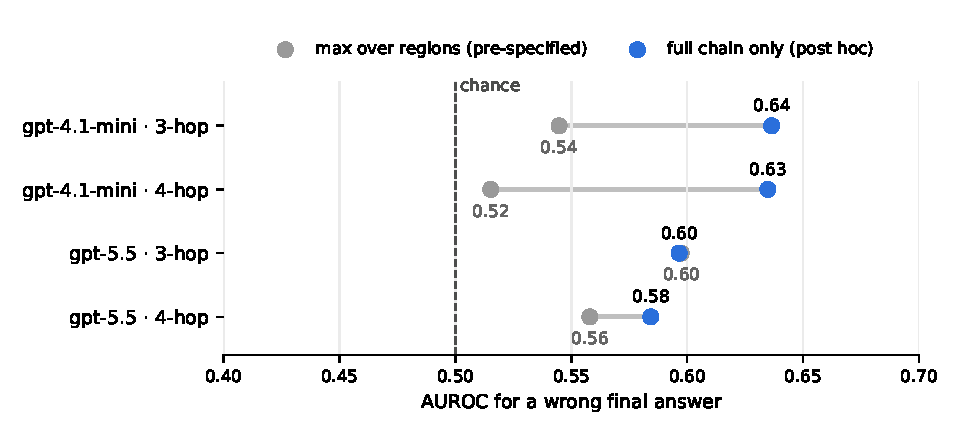
\includegraphics[width=0.85\linewidth]{fig_aggregator.pdf}
\caption{AUROC of the composition score for a wrong final answer on scale300 3- and 4-hop
questions (about 100 per row): the pre-specified maximum over regions against the
full-chain region alone. Computed after the pre-specified analysis.}
\label{fig:agg}
\end{figure}

Swapping the full-chain score into the H1 model gives Table~\ref{tab:full}.

\begin{table}[h]
\centering
\small
\caption{Exploratory H1 with the full-chain composition score.}
\label{tab:full}
\begin{tabular}{llrl}
\toprule
Model & Subset & Comp. AUROC (full chain) & H1 gain, 95\% CI \\
\midrule
gpt-4.1-mini & all 292 & 0.656 & $+0.030$ [$-0.018$, +0.077] \\
gpt-4.1-mini & 3--4 hop & 0.638 & $\mathbf{+0.053}$ [+0.006, +0.102] \\
gpt-5.5 & all 300 & 0.598 & $+0.003$ [$-0.013$, +0.018] \\
gpt-5.5 & 3--4 hop & 0.587 & $-0.006$ [$-0.021$, +0.008] \\
\bottomrule
\end{tabular}
\end{table}

This was found after looking at the results, so it is a hypothesis, not a finding. It is
worth pre-registering because the mechanism is specific and checkable: the sub-region
prompts fail, not the idea of composition. gpt-5.5 stays null under either score.

\section{Discussion and limitations}

The evidence answers the parent project's first question clearly and the second only partly.
Stated confidence is a poor guide for choosing checks in every open-book run, so a better
signal is needed. Composition is a candidate: it beat confidence-based selection on every
two-hop pilot and carries real localisation signal (H2 AUROC 0.59--0.64). But at scale and
as pre-specified it is not better than plain self-consistency, which costs the same number
of calls and needs no decomposition. Three patterns are consistent across runs:
\begin{itemize}
  \item \textbf{Weaker models show the signal more.} gpt-4.1-mini is where composition adds
        information. For gpt-4.1 and gpt-5.5, same-route noise and self-consistency already
        capture it.
  \item \textbf{It is an evidence-chaining signal.} It vanishes in closed book, where
        confidence takes over.
  \item \textbf{The sample count is not the lever.} $N = 3$ already gives what $N = 10$
        gives, which keeps the probe cheap if it is used at all.
\end{itemize}

\paragraph{Limitations.}
\begin{itemize}
  \item \textbf{Answer identity.} Exact-match normalisation counts paraphrases as
        disagreement. That inflates composition on correct answers (about 125 of 300
        questions are inconsistent but correct) and dilutes the signal.
  \item \textbf{Synthetic sub-region prompts.} Nested composites for 3- and 4-hop sub-regions
        are awkward and saturate the score (Section~5).
  \item \textbf{Labels.} Automatic token-F1 labels miss valid paraphrases and cannot tell an
        unsupported claim from a valid inference on a false premise. Nothing was
        hand-labelled.
  \item \textbf{Audit.} 218 of 300 scale300 questions carry audit flags (mostly awkwardly
        rendered knowledge-base hops), and none were reviewed by hand.
  \item \textbf{One dataset, train split.} Everything is MuSiQue train and no held-out
        evaluation has been run, so all results are development results.
  \item \textbf{Probe cost sits outside the budget.} Stage F treats probe calls as free
        alongside a fixed number of checks, while a real deployment pays for both.
  \item \textbf{Temperature.} All models ran at 0.7. gpt-5.5 needed reasoning switched off
        to allow it, so its reasoning mode is untested.
\end{itemize}

\section{Next steps}

Fix the two measurement problems first, then rerun the pre-registered test on held-out
data. Only then is the budget-allocation problem worth solving. Steps 1--3 need no new API
calls, since every sample is cached.
\begin{enumerate}
  \item \textbf{Answer-equivalence judge (no new probes).} A gold-free judge (alias lists
        plus a cheap model asked whether two answers name the same thing) merges paraphrases
        before scoring. Re-score all cached runs and check how many of the roughly 125
        ``inconsistent but correct'' questions remain.
  \item \textbf{Pre-register the aggregator.} Freeze the full-chain score (or a mean over
        regions) as the primary composition feature, and use sub-region scores only for H2
        localisation. Write it down before step 4.
  \item \textbf{Hand audit and spot labels.} Review the 218 flagged scale300 questions and
        hand-label about 50 disagreements, to measure label error and drop broken hop
        renderings. Re-scoring after the audit is free.
  \item \textbf{Held-out confirmation.} Draw a fresh set from MuSiQue dev (2-, 3- and 4-hop),
        run gpt-4.1-mini and gpt-5.5 with the frozen protocol, and test H1 once. Add a second
        dataset (2WikiMultiHopQA) if the effect holds.
  \item \textbf{Model sweep.} Add gpt-4o-mini, gpt-5.4-nano, gpt-5.4-mini and the Groq
        gpt-oss-120b pilot (due around 18--19 November) to test whether the effect tracks
        model strength.
  \item \textbf{Budget allocation, only if step 4 is positive.} Put probes and checks in one
        budget, $B = c \cdot \text{checks} + \text{calls}$, and choose which questions to
        probe and how many checks remain. The cached $N = 3, 5, 10$ runs let the frontier be
        computed offline for any cost ratio $c$. Since $N = 3$ is enough, the useful lever
        is probe coverage: probe only questions where self-consistency is ambiguous.
  \item \textbf{Feed real chains back to the parent model.} The measured error and
        propagation rates on these chains (for example 34--47\% final-answer error on
        gpt-4.1-mini) can replace or check the PARC-fitted constants in
        \code{dag\_codes/constants.py}.
\end{enumerate}

\appendix
\section{Reproducibility}

All code is in \code{will/project1/}. Every API response is cached under
\code{cache/openai/<model>/}, so any analysis below reruns at no cost.

\begin{center}
\small
\begin{tabular}{lp{0.58\linewidth}}
\toprule
File & What it does \\
\midrule
\code{01\_build\_pilot.py} & Stage A: select linear chains, render steps, write tasks, gold and audit sheet \\
\code{02\_generate\_original.py} & Stage B: original answer, step answers, confidence \\
\code{03\_run\_probes.py} & Stage C: probes, same-route control, self-consistency \\
\code{04\_label.py} & Stage D: the only stage that reads gold answers \\
\code{05\_analyze.py} & Stage E: H1 and H2 \\
\code{06\_budget.py} & Stage F: the parent project's fixed-budget evaluation \\
\code{summarize\_runs.py} & one table across all runs \\
\code{run\_openai.sh} & runner: \code{check}, \code{replicate}, \code{build}, \code{run}, \code{analyze}, \code{smoke} \\
\code{paper/make\_figures.py} & regenerates Figure~\ref{fig:agg} from the cached runs \\
\bottomrule
\end{tabular}
\end{center}

\begin{verbatim}
cd will/project1
./run_openai.sh run pilot100                     # gpt-4.1 by default
TBYT_MODEL=gpt-4.1-mini TBYT_SAMPLES_PER_ROUTE=5 ./run_openai.sh run pilot100
TBYT_MODEL=gpt-5.5 TBYT_REASONING_EFFORT=none ./run_openai.sh run scale300
python3 summarize_runs.py
python3 paper/make_figures.py
\end{verbatim}

Each run writes to \code{outputs\_openai/runs/<set>\_\_<model>\_\_<condition>\_\_n<N>/}, with
a config snapshot per stage. Total-variation scores are summed in a fixed order and rounded
to 10 decimals, so replays are bit-identical. The Groq pilot (\code{outputs/}) shares the
code and is unaffected.

\end{document}
